\RequirePackage[l2tabu,orthodox]{nag}
%
\documentclass[12pt, a4paper]{report}
%
\usepackage[utf8]{inputenc}
\usepackage[T1,T2A]{fontenc}
\usepackage[russian]{babel}
%
\usepackage[intlimits]{amsmath}  % Basic math structures
\usepackage{amssymb}  % Extended symbols
\usepackage{amsthm}  % Theorem environment
\usepackage{bm}
%
\usepackage[a4paper,margin=3cm,includefoot,heightrounded]{geometry}
\usepackage[colorlinks,unicode]{hyperref}
\usepackage{layout}
\usepackage{dsfont}
\usepackage{mathrsfs}
\usepackage{mathtools}
\usepackage{multirow}
\usepackage{tikz}
\usepackage{titlesec}
\usepackage{pgf}
\usepackage{pgfplots}
\usepackage{graphicx}
%
\usepackage{wrapfig}
%
\graphicspath{ {./int-figs/} }
%
\pgfplotsset{compat=1.16}
%
%
\titleformat{\chapter}[block]{\normalfont\huge\bfseries\centering}{\S \thechapter.}{20pt}{\Huge}
\newcommand*{\CC}{\mathbb{C}}
\newcommand*{\RR}{\mathds{R}}
\newcommand*{\ZZ}{\mathds{Z}}
\newcommand*{\NN}{\mathds{N}}
\newcommand*{\QQ}{\mathds{Q}}

\newcommand*{\EV}{\mathbf{E}}
\newcommand*{\Var}{\mathbf{D}}
\newcommand*{\PR}{\mathbf{P}}

\newcommand*{\D}{\bm{D}}
\newcommand*{\R}{\bm{R}}
\newcommand{\BraceThree}{%
	\multirow{3}{*}{$\left\{\begin{array}{@{}l@{}} \null \\ \null \\ \null\end{array}\right.$}%
}

\newcommand{\BraceTwo}{%
	\multirow{2}{*}{$\left\{\begin{array}{@{}l@{}} \null \\ \null\end{array}\right.$}%
}

\renewcommand\qedsymbol{$\blacksquare$}

\theoremstyle{plain}
\newtheorem{Th}{Теорема}
\newtheorem*{Th*}{Теорема}
\newtheorem{Lem}{Лемма}
\newtheorem*{Lem*}{Лемма}
\newtheorem*{St}{Утверждение}
\newtheorem*{Prop}{Свойства}

\theoremstyle{definition}
\newtheorem*{Def}{Определение}
\newtheorem*{Ex}{Пример}
\newtheorem*{Nam}{Обозначение}
\newtheorem*{Agr}{Договоренность}

\theoremstyle{remark}
\newtheorem*{Rem}{Замечание}
\newtheorem*{Probl}{Упражнение}

\renewcommand{\proofname}{Доказательство}
\addto\captionsrussian{
	\renewcommand{\proofname}{Доказательство}
}

\newenvironment{amatrix}[1]{%
	\left(\begin{array}{@{}*{#1}{c}|c@{}}
	}{%
	\end{array}\right)
}

\DeclareMathOperator*{\Res}{Res}
\DeclareMathOperator{\PE}{E}
\DeclareMathOperator{\PP}{P}

\renewcommand{\Re}{\operatorname{Re}}
\renewcommand{\Im}{\operatorname{Im}}

\DeclareMathOperator*{\argmin}{arg\,min}
%
\begin{document}
%
\thispagestyle{empty}
\sloppy
\begin{titlepage}
\begin{center}
Московский государственный университет имени~М.~В.~Ломоносова\\
механико-математический факультет\\
кафедра математической статистики и случайных процессов\\


\centering
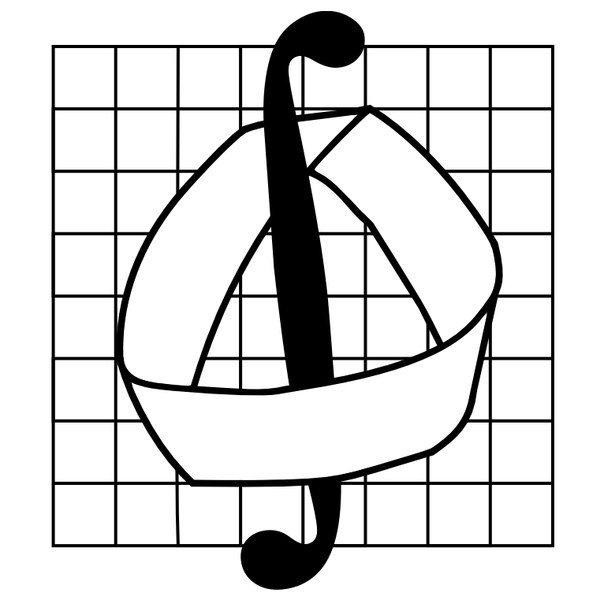
\includegraphics[width=0.3\textwidth]{mechmath.jpg}


\vspace*{100pt} Курсовая работа\\студента 403 группы \\
Купрякова Василия Юрьевича
\\
\vspace{10pt} {\Large{\textbf{Непараметрическая оценка плотности мультипликативно зашумленных данных}}\\}

\vspace*{40pt}

\begin{flushright}
Научный руководитель:\\ с.н.с., к.ф.-м.н.\\  Шкляев Александр Викторович\\
\end{flushright}

\vspace*{\fill} Москва, 2020
\end{center}
\end{titlepage}
\clearpage
%
\tableofcontents
%
\chapter{Введение}
В работу мы изучим задачу, которая возникает при исследовании примесий в жидкости.

Примеси в исследуемой жидкости --- это движущиеся частицы с размерами порядка $10^{-8}$ м.
Жидкость просвечивают лазером, а камера фиксирует частицы, которые попали в луч.

Получается последовательность изображений. Для каждой частицы эта последовательность является
последовательностью проекций частиц на площадь камеры. Мы можем построить векторы перемещений
частиц в проекции на плоскость камеры по этим снимкам. Для отдельной частицы такие перемещения
образуют броуновское движение с нулевым сносом и дисперсией $\sigma^2 = c/d$, где $c$ --- некоторая
константа, а $d$ --- размер частицы.

Проблема в том, что размер частицы не связан напрямую с размером ее изображения. Наша задача ---
оценить распределение истинных размеров частиц по размерам на снимках.

Будем изучать равносильную задачу: оценить распределение $\sigma^2$.
Рассмотрим $n$ случайно выбранных частиц $E_1, \dots, E_n$. Обозначим дисперсии для
их движения как $\sigma_1^2, \dots, \sigma_n^2$. Для $i$-й частицы у нас есть два
$k(i)$-мерных вектора перемещений: $A_i^1, \dots, A_i^{k(i)}$ по оси $x$ 
и $A_i^{k(i)+1}, \dots, A_i^{2k(i)}$ по оси $y$. Мы будем рассматривать только частный случай,
когда все $k(i)$ равны $k$, а $\sigma_i^2$ непрерывна.

$A_i^1, \dots, A_i^{2k}$ условно независимы при условии $\sigma_i^2$ и имеют условное
распределение $\mathcal{N}\left(0, \sigma_i^2\right)$. Дальше вместо выборки
$A_i^1, \dots, A_i^{2k}$ будем рассматривать достаточную статистику $Z_i = \sum\limits_{j=1}^{2k} \left(A_i^j\right)^2$.
Заметим далее, что $Z_i = \sigma_i^2 Y_i$, где $Y_i \sim \chi^2_{2k}$.
При этом, $Y_i$ независимы и не зависят от дисперсии $\sigma_i^2$.

Обозначим $X_i = \sigma_i^2$. Тогда задачу можно сформулировать так:
$X_1, \dots, X_n$ --- независимые одинаково распределенные случайные величины
с неизвестным распределением и положительным носителем; 
$Y_1, \dots, Y_n$ --- независимые от них н.о.р. с.в. с распределением $\chi^2_{2k}$;
$Z_1, \dots, Z_n = X_1 Y_1, \dots, X_n Y_n$ --- наблюдаемые случайные величины;
а сама задача --- по наблюдениям $Z_1, ..., Z_n$ оценить распределение $X_1$.
%
\section{Правильная часть ряда Лорана для $f(z) = e^{az} e^{-1/(2s^2)} e^{n/s}$}
\begin{Th*}
Пусть $k \ge 0$; пусть
\[
    f(z) = e^{az} e^{-1/(2s^2)} e^{b/z}
\]
Тогда $k$-й член ряда Лорана для $f$ равен
\[
    \sum_{l=0}^{\infty}
    \sum_{m=0}^{\infty} \frac{a^{2m+k+l} / \left( -2 \right)^m}{(2m+k+l)!\,m!} \\
    \frac{n^l}{l!}
\]
\end{Th*}
\begin{proof}
Определим
\begin{align*}
    & g(t) = e^{az} e^{-1/(2s^2)} \\
    & h(t) = e^{b/z}
\end{align*}
Обе функции голоморфны в $\CC \setminus \{0\}$. Поэтому их ряды сходятся абсолютны и мы можем умножить ряды по Коши, чтобы получить ряд Лорана для $f$.

У функции $e^{n/s}$ правильная часть константна.
Поэтому, согласно теореме о правильной части произведения голоморфной функции и функции с константной правильной частью, 
нам достаточно знать только правильную часть разложения функции $g$, которую мы нашли в предыдущей теореме.

Пусть $\{\alpha_n\}_{n=-\infty}^\infty$ --- коэффициенты для $g$, а $\{\beta_n\}_{n=-\infty}^0$ --- коэффициенты для $h$, а $\{\gamma_n\}_{n=-\infty}^\infty$ --- коэффициенты $f$.
Для наглядности, приведем формулу $k$-го члена их произведения, где $k \ge 0$:
\[
    \gamma_k =
    \sum_{l=-\infty}^{0} \alpha_{k-l} \beta_l =
    \sum_{l=0}^{\infty} \alpha_{k+l} \beta_{-l}
\]
Приведем также формулы для $\alpha_k$ и $\beta_{-k}$:
\begin{align*}
    & \alpha_k = \sum_{m=0}^{\infty} \frac{a^{2m+k} / \left( -2 \right)^m}{(2m+k)!\,m!} \\
    & \beta_{-k} = \frac{n^k}{k!}
\end{align*}
Подставим $\alpha_k$ и $\beta_{-k}$ в формулу для $\gamma_k$:
\[
    \gamma_k =
    \sum_{l=0}^{\infty} \alpha_{k+l} \beta_{-l} =
%
    \sum_{l=0}^{\infty}
    \sum_{m=0}^{\infty} \frac{a^{2m+k+l} / \left( -2 \right)^m}{(2m+k+l)!\,m!} \\
    \frac{n^l}{l!}
\]
\end{proof}

%
\chapter{Вычисление обратного преобразования Лапласа с помощью формулы Меллина и основной теоремы о вычетах}

Мы выразили $g_{m,n}(t)$ как:
\begin{equation}\label{eq:gmn}
    g_{m,n}(t) = 
    \frac{1}{t^{k-1}} \frac{\Gamma(k)}{\sqrt{2^m}} L^{-1}_u \left[ \frac{1}{u^k} \psi_{m,n} \left( \frac{1}{2^{m+1} u} - n \right) \right] (t)
\end{equation}

Теперь нужно вычислить обратное преобразование Лапласа. Для этого мы будем использовать формулу Меллина:
\[
    L^{-1}_s \left[ F \left( s \right)  \right](t) = 
    \frac{1}{2\pi i} \int_{\alpha - i \infty}^{\alpha + i \infty} e^{ts} F(s) ds
\]

Итак, нам нужно вычислить:
\[
    L^{-1}_u \left[ \frac{1}{u^k} \psi_{m,n} \left( \frac{1}{2^{m+1} u} - n \right) \right] (t)
\]

Подставим вместо $\psi$ формулу нашего вейвлета:
\[
    L^{-1}_u \left[ \frac{1}{u^k} \psi_{m,n} \left( \frac{1}{2^{m+1} u} - n \right) \right] (t) =
%
    L^{-1}_u \left[ \frac{1}{u^k} \frac{2}{\sqrt{3} \pi^{1/4} } 
    \left( 1 - \left( \frac{1}{2^{m+1} u} - n \right)^2 \right) 
    \exp \left( -\frac{1}{2} \left( \frac{1}{2^{m+1}u} - n \right)^2  \right)
    \right](t)
\]

Распишем множитель перед экспонентой:
\[
    1 - \left( \frac{1}{2^{m+1} u } - n \right)^2 =
    1 - \left( \frac{1}{2^{2(m+1)} u^2} - 2 \frac{1}{2^{m+1} u } n + n^2 \right) =
    \left( 1 - n^2 \right) + \frac{1}{u} \left(\frac{n}{2^m}\right) - \frac{1}{u^2} \left(\frac{1}{4^{m+1}}\right)
\]

Введем обозначение:
\[
    r_{m,n}(u) = \frac{2}{\sqrt{3} \pi^{1/4}} \exp \left( -\frac{1}{2} \left( \frac{1}{2^{m+1}u} - n \right)  \right) 
\]

Таким образом,
\begin{multline}\label{eq:invlap_gen}
    L^{-1}_u \left[ \frac{1}{u^k} \psi_{m,n} \left( \frac{1}{2^{m+1} u} - n \right) \right] (t) =
    \left( 1 - n^2 \right)  L^{-1}_u \left[ \frac{1}{u^k} r_{m,n}(u) \right](t) +
    \left( \frac{n}{2^m} \right)  L^{-1}_u \left[ \frac{1}{u^{k+1}} r_{m,n}(u) \right](t)
-\\-
    \left( \frac{1}{4^{m+1}} \right)  L^{-1}_u \left[ \frac{1}{u^{k+2}} r_{m,n}(u) \right](t)
\end{multline}

Отсюда видно, что достаточно найти $L^{-1}_u [\frac{1}{u^k} r_{m,n}(u)](t)$ для каждого $k$.

\section{Находим $L^{-1}_u [\frac{1}{u^k} r_{m,n}(u)](t)$}
Выше мы ввели
\[
    L^{-1}_u \left[ \frac{1}{u^k} r_{m,n}(u) \right](t)
\]
Подставим обратно $r_{m,n}(u)$:
\[
    L^{-1}_u \left[ \frac{1}{u^k} r_{m,n}(u) \right](t) =
%
    L^{-1}_u \left[ \frac{1}{u^k} \frac{2}{\sqrt{3} \pi^{1/4} } 
    \exp \left( -\frac{1}{2} \left( \frac{1}{2^{m+1}u} - n \right)^2  \right)
    \right](t)
\]
Раскроем квадрат под экспонентой:
\[
    L^{-1}_u \left[ \frac{1}{u^k} r_{m,n}(u) \right](t) =
%
    L^{-1}_u \left[ \frac{1}{u^k} \frac{2}{\sqrt{3} \pi^{1/4} } 
    \exp \left( -\frac{1}{2}
    \left(\left( n^2 \right) - \frac{1}{u} \left(\frac{n}{2^m}\right) + \frac{1}{u^2} \left(\frac{1}{4^{m+1}}\right)\right)
    \right)
    \right](t)
\]
Сгруппируем $2^{m+1}u$:
\[
    L^{-1}_u \left[ \frac{1}{u^k} r_{m,n}(u) \right](t) =
%
    L^{-1}_u \left[ \frac{2^{k(m+1)}}{\left(2^{m+1}u\right)^k} \frac{2}{\sqrt{3} \pi^{1/4} } 
    \exp \left( -\frac{n^2}{2} + \frac{n}{2^{m+1}u} - \frac{1}{2 \left( 2^{m+1}u \right)^2 }
    \right)
    \right](t)
\]
Вынесем множители, не зависящие от $u$, за $L^{-1}_u$:
\[
    L^{-1}_u \left[ \frac{1}{u^k} r_{m,n}(u) \right](t) =
%
    e^{-\frac{n^2}{2}} 2^{k(m+1)} \frac{2}{\sqrt{3} \pi^{1/4}}
    L^{-1}_u \left[ \frac{1}{\left(2^{m+1}u\right)^k}
    \exp \left(\frac{n}{2^{m+1}u} - \frac{1}{2 \left( 2^{m+1}u \right)^2 }
    \right)
    \right](t)
\]
Используя теорему о замене переменной в обратном преобразовании Лапласа, делаем замену $s=2^{m+1}u$:
\[
    L^{-1}_u \left[ \frac{1}{u^k} r_{m,n}(u) \right](t) =
%
    e^{-\frac{n^2}{2}} 2^{(k-1)(m+1)} \frac{2}{\sqrt{3} \pi^{1/4}}
    L^{-1}_s \left[ \frac{1}{s^k}
    \exp \left(\frac{n}{s} - \frac{1}{2 s^2 }
    \right)
    \right] \left( \frac{t}{2^{m+1}} \right)
\]
\section{Находим обратное преобразование Лапласа}
В предыдущем разделе мы выразили:
\begin{equation}\label{eq:invlap}
    L^{-1}_u \left[ \frac{1}{u^k} r_{m,n}(u) \right](t) =
%
    e^{-\frac{n^2}{2}} 2^{(k-1)(m+1)} \frac{2}{\sqrt{3} \pi^{1/4}}
    L^{-1}_s \left[ \frac{1}{s^k}
    \exp \left(\frac{n}{s} - \frac{1}{2 s^2 }
    \right)
    \right] \left( \frac{t}{2^{m+1}} \right)
\end{equation}
Чтобы вычислить правую часть, найдем теперь
\begin{equation}\label{eq:invlap_as_int}
    L^{-1}_s \left[ \frac{1}{s^k}
    \exp \left(\frac{n}{s}\right)
    \exp \left(-\frac{1}{2 s^2 }\right)
    \right] \left( \tau \right)
\end{equation}
Воспользуемся формулой Меллина обратного преобразования Лапласа. У наc особенность только в нуле, поэтому можно взять любую $\alpha>0$:
\[
    L^{-1}_s \left[ \frac{1}{s^k}
    \exp \left(\frac{n}{s}\right)
    \exp \left(-\frac{1}{2 s^2 }\right)
    \right] \left( \tau \right) =
%
    \frac{1}{2\pi i}\int_{\alpha-i\infty}^{\alpha+i\infty} e^{s\tau} \frac{1}{s^k} e^{-1/(2s^2)} e^{n/s} ds
\]

\usetikzlibrary{arrows}
\usetikzlibrary{decorations.markings}
\usetikzlibrary{patterns}
%
%
\begin{tikzpicture}
    \begin{axis} [
        axis on top,
        axis lines=middle,
        xmin=-5,
        xmax=5,
        ymin=-5,
        ymax=5,
        unit vector ratio=1 1 1
        ]
%
%        \fill[pattern=north west lines, opacity=0.6] (-10,10) rectangle (2,-10);
%        \fill[white] (2, -3) -- (2, 3) arc(90:270:3) -- cycle;
%        \draw[dashed] (2, -10) -- (2, -3) arc(270:90:3) -- (2,10);
%
%
        \begin{scope}[decoration={
            markings,
            mark=between positions 0 and 1 step 5mm with {\arrow {stealth}}}
            ]
%
            \draw [postaction=decorate] (2,-4) -- (2,4) -- plot [domain=1:3, variable=\t] ({2 + 4*cos(\t * pi / 2 r)}, {4*sin(\t * pi / 2 r)}) -- cycle;
        \end{scope}
        \draw[fill=black] (0, 0) circle (2pt);
    \end{axis}
\end{tikzpicture}
%


Берем контур $C$ = $C_1 + C_2$, где $C_1$ --- искомый, а $C_2$ --- дуга окружности (слева от $C_1$ с центром в $(\alpha, 0)$).

Оценим $F(s) := (1/s^k) e^{-1/(2s^2)} e^{n/s}$ на $C_r$, где $r > 4\alpha$. Для этого оценим каждый из множителей. Сначала $1/s$:
\[
    \left|\frac{1}{s}\right| = 
    \left|\frac{1}{\alpha+re^{i\phi}}\right| =
    \frac{1}{\sqrt{\left(\alpha+r\cos\phi\right)^2 + \left(r\sin\phi\right)^2}} =
    \frac{1}{r\sqrt{\left(\frac{\alpha}{r} + \cos\phi\right)^2 + \sin^2\phi}} \le
    \frac{1}{r\sqrt{1 + \frac{2\alpha\cos\phi}{r}}} \le
    \frac{1}{r\sqrt{1 + \frac{\cos\phi}{2}}} \le
    \frac{\sqrt{2}}{r} 
\]
Теперь оценим $e^{-1/(2s^2)}$ на том же контуре. Известно, что $|e^{z}| = e^{|z|}$
\[
    \left|\exp\left(-\frac{1}{2s^2}\right)\right| \le
    \exp\left(\left|-\frac{1}{2s^2}\right|\right) =
    \exp\left(\frac{1}{r^2}\right)
\]
Аналогично оцениваем $e^{n/s}$:
\[
    \left| \exp\left( \frac{n}{s} \right)  \right| \le 
    \exp\left(\left| \frac{n}{s} \right|\right) =
    \exp\left( \frac{|n|\sqrt{2} }{r} \right) 
\]
Объединяем оценки и получаем:
\[
    \left|\frac{1}{s^k} \exp\left(-\frac{1}{2s^2}\right) \exp\left(\frac{n}{s}\right)\right| \le
    \left(\frac{\sqrt{2}}{r}\right)^k \exp\left(\frac{1}{r^2}\right) \exp\left(\frac{|n|\sqrt{2}}{r}\right)
    \xrightarrow[r \to \infty]{} 0
\]

А значит, по лемме Жордана $\int\limits_{C_r} e^{s\tau} F(s)ds$ стремится к нулю.
Поэтому можем использовать основную теорему о вычетах:
\[
    \frac{1}{2\pi i}\int_{\alpha-i\infty}^{\alpha+i\infty} e^{s\tau} \frac{1}{s^k} e^{-1/(2s^2)} e^{n/s} ds =
    \frac{1}{2\pi i} 2\pi i \Res_0 \left( e^{s\tau} \frac{1}{s^k} e^{-1/(2s^2)} e^{n/s} ds \right)
\]
У нас возникает два случая: $n=0$ и $n\neq$0
\subsection{Случай $n = 0$}
Воспользуемся теоремой о правильной части функции $e^{s\tau} e^{-1/(2s^2)}$. Нам нужен $k-1$-й член ряда Лорана. Получаем:
\[
    \frac{1}{2\pi i}\int_{\alpha-i\infty}^{\alpha+i\infty} e^{s\tau} \frac{1}{s^k} e^{-1/(2s^2)} e^{n/s} ds =
    \sum_{j=0}^{\infty} \frac{\tau^{2j+k-1} / (-2)^j}{(2j+k-1)!\,j!}
\]
Таким образом, мы выразили вычислили \ref{eq:invlap_as_int}:
\[
    L^{-1}_s \left[ \frac{1}{s^k}
    \exp \left(\frac{n}{s}\right)
    \exp \left(-\frac{1}{2 s^2 }\right)
    \right] \left( \tau \right)
=
    \sum_{j=0}^{\infty} \frac{\tau^{2j+k-1} / (-2)^j}{(2j+k-1)!\,j!}
\]
Подставим это выражение в \ref{eq:invlap}, заменяя $\tau$ на $t/2^{m+1}$:
\begin{multline*}
    L^{-1}_u \left[ \frac{1}{u^k} r_{m,n}(u) \right](t) =
%
    e^{-\frac{n^2}{2}} 2^{(k-1)(m+1)} \frac{2}{\sqrt{3} \pi^{1/4}}
    L^{-1}_s \left[ \frac{1}{s^k}
    \exp \left(\frac{n}{s} - \frac{1}{2 s^2 }
    \right)
    \right] \left( \frac{t}{2^{m+1}} \right) =
\\%
    e^{-\frac{n^2}{2}} 2^{(k-1)(m+1)} \frac{2}{\sqrt{3} \pi^{1/4}}
    \sum_{j=0}^{\infty} \frac{\left(\frac{t}{2^{m+1}}\right)^{2j+k-1} / (-2)^j}{(2j+k-1)!\,j!}
\end{multline*}
Наконец, подставим это в~\ref{eq:invlap_gen}:
\begin{multline}
    L^{-1}_u \left[ \frac{1}{u^k} \psi_{m,n} \left( \frac{1}{2^{m+1} u} - n \right) \right] (t) =
    \left( 1 - n^2 \right)  L^{-1}_u \left[ \frac{1}{u^k} r_{m,n}(u) \right](t) +
    \left( \frac{n}{2^m} \right)  L^{-1}_u \left[ \frac{1}{u^{k+1}} r_{m,n}(u) \right](t) +
\\+
    \left( \frac{1}{4^{m+1}} \right)  L^{-1}_u \left[ \frac{1}{u^{k+2}} r_{m,n}(u) \right](t)
=\\=
    \left( 1-n^2 \right) 
    e^{-\frac{n^2}{2}} 2^{(k-1)(m+1)} \frac{2}{\sqrt{3} \pi^{1/4}}
    \sum_{j=0}^{\infty} \frac{\left(\frac{t}{2^{m+1}}\right)^{2j+k-1} / (-2)^j}{(2j+k-1)!\,j!}
+
    \left( \frac{n}{2^m} \right) 
    e^{-\frac{n^2}{2}} 2^{k(m+1)} \frac{2}{\sqrt{3} \pi^{1/4}}
    \sum_{j=0}^{\infty} \frac{\left(\frac{t}{2^{m+1}}\right)^{2j+k} / (-2)^j}{(2j+k)!\,j!}
-\\-
    \left( \frac{1}{4^{m+1}} \right) 
    e^{-\frac{n^2}{2}} 2^{(k+1)(m+1)} \frac{2}{\sqrt{3} \pi^{1/4}}
    \sum_{j=0}^{\infty} \frac{\left(\frac{t}{2^{m+1}}\right)^{2j+k+1} / (-2)^j}{(2j+k+1)!\,j!}
\end{multline}
Теперь получим выражение для $g(t)$, подставляя только что полученную формулу в~\ref{eq:gmn}:
\begin{multline*}
    g_{m,n}(t) = 
    \frac{1}{t^{k-1}} \frac{\Gamma(k)}{\sqrt{2^m}} L^{-1}_u \left[ \frac{1}{u^k} \psi_{m,n} \left( \frac{1}{2^{m+1} u} - n \right) \right] (t)
=\\=
    \frac{1}{t^{k-1}} \frac{\Gamma(k)}{\sqrt{2^m}} \left( 1-n^2 \right) 
    e^{-\frac{n^2}{2}} 2^{(k-1)(m+1)} \frac{2}{\sqrt{3} \pi^{1/4}}
    \sum_{j=0}^{\infty} \frac{\left(\frac{t}{2^{m+1}}\right)^{2j+k-1} / (-2)^j}{(2j+k-1)!\,j!}
+\\+
    \frac{1}{t^{k-1}} \frac{\Gamma(k)}{\sqrt{2^m}} \left( \frac{n}{2^m} \right) 
    e^{-\frac{n^2}{2}} 2^{k(m+1)} \frac{2}{\sqrt{3} \pi^{1/4}}
    \sum_{j=0}^{\infty} \frac{\left(\frac{t}{2^{m+1}}\right)^{2j+k} / (-2)^j}{(2j+k)!\,j!}
-\\-
    \frac{1}{t^{k-1}} \frac{\Gamma(k)}{\sqrt{2^m}} \left( \frac{1}{4^{m+1}} \right) 
    e^{-\frac{n^2}{2}} 2^{(k+1)(m+1)} \frac{2}{\sqrt{3} \pi^{1/4}}
    \sum_{j=0}^{\infty} \frac{\left(\frac{t}{2^{m+1}}\right)^{2j+k+1} / (-2)^j}{(2j+k+1)!\,j!}
\end{multline*}
%
Начнем упрощать выражение. Для начала, вынесем из суммы, степень, не зависящую от переменной суммирования и сделаем замену $n=0$ (так как рассматриваем именно этот случай):
\[
    g_{m,0}(t) =
%
    \frac{\Gamma(k)}{\sqrt{2^m}}
    \frac{2}{\sqrt{3} \pi^{1/4}} \left(
%
    \sum_{j=0}^{\infty} \frac{\left(\frac{t}{2^{m+1}}\right)^{2j} / (-2)^j}{(2j+k-1)!\,j!}
-
    \left( \frac{t^2}{4^{m+1}} \right) 
    \sum_{j=0}^{\infty} \frac{\left(\frac{t}{2^{m+1}}\right)^{2j} / (-2)^j}{(2j+k+1)!\,j!}
%
    \right)
\]
\subsection{Случай $n \neq 0$}
Воспользуемся теоремой о правильной части функции $e^{s\tau} e^{-1/(2s^2)} e^{n/s}$. Нам нужен $k-1$-й член ряда Лорана. Получаем:
\[
    \frac{1}{2\pi i}\int_{\alpha-i\infty}^{\alpha+i\infty} e^{s\tau} \frac{1}{s^k} e^{-1/{2s^2}} e^{n/s} ds =
    \sum_{i=0}^{\infty} \sum_{j=0}^{\infty} \frac{\tau^{2j+k-1+i} / (-2)^j}{(2j+k-1+i)!\,j!} \frac{n^i}{i!}
\]
Таким образом, мы выразили вычислили \ref{eq:invlap_as_int}:
\[
    L^{-1}_s \left[ \frac{1}{s^k}
    \exp \left(\frac{n}{s}\right)
    \exp \left(-\frac{1}{2 s^2 }\right)
    \right] \left( \tau \right)
=
    \sum_{i=0}^{\infty} \sum_{j=0}^{\infty} \frac{\tau^{2j+k-1+i} / (-2)^j}{(2j+k-1+i)!\,j!} \frac{n^i}{i!}
\]
Подставим это выражение в \ref{eq:invlap}, заменяя $\tau$ на $t/2^{m+1}$:
\begin{multline*}
    L^{-1}_u \left[ \frac{1}{u^k} r_{m,n}(u) \right](t) =
%
    e^{-\frac{n^2}{2}} 2^{(k-1)(m+1)} \frac{2}{\sqrt{3} \pi^{1/4}}
    L^{-1}_s \left[ \frac{1}{s^k}
    \exp \left(\frac{n}{s} - \frac{1}{2 s^2 }
    \right)
    \right] \left( \frac{t}{2^{m+1}} \right) =
\\%
    e^{-\frac{n^2}{2}} 2^{(k-1)(m+1)} \frac{2}{\sqrt{3} \pi^{1/4}}
    \sum_{i=0}^{\infty} \sum_{j=0}^{\infty} \frac{\left( \frac{t}{2^{m+1}} \right) ^{2j+k-1+i} / (-2)^j}{(2j+k-1+i)!\,j!} \frac{n^i}{i!}
\end{multline*}
Наконец, подставим это в~\ref{eq:invlap_gen}:
\begin{multline}
    L^{-1}_u \left[ \frac{1}{u^k} \psi_{m,n} \left( \frac{1}{2^{m+1} u} - n \right) \right] (t) =
    \left( 1 - n^2 \right)  L^{-1}_u \left[ \frac{1}{u^k} r_{m,n}(u) \right](t) +
    \left( \frac{n}{2^m} \right)  L^{-1}_u \left[ \frac{1}{u^{k+1}} r_{m,n}(u) \right](t)
+\\+
    \left( \frac{1}{4^{m+1}} \right)  L^{-1}_u \left[ \frac{1}{u^{k+2}} r_{m,n}(u) \right](t)
=\\=
    \left( 1-n^2 \right) 
    e^{-\frac{n^2}{2}} 2^{(k-1)(m+1)} \frac{2}{\sqrt{3} \pi^{1/4}}
    \sum_{i=0}^{\infty} \sum_{j=0}^{\infty} \frac{\left( \frac{t}{2^{m+1}} \right) ^{2j+k-1+i} / (-2)^j}{(2j+k-1+i)!\,j!} \frac{n^i}{i!}
+\\+
    \left( \frac{n}{2^m} \right) 
    e^{-\frac{n^2}{2}} 2^{k(m+1)} \frac{2}{\sqrt{3} \pi^{1/4}}
    \sum_{i=0}^{\infty} \sum_{j=0}^{\infty} \frac{\left( \frac{t}{2^{m+1}} \right) ^{2j+k+i} / (-2)^j}{(2j+k+i)!\,j!} \frac{n^i}{i!}
-\\-
    \left( \frac{1}{4^{m+1}} \right) 
    e^{-\frac{n^2}{2}} 2^{(k+1)(m+1)} \frac{2}{\sqrt{3} \pi^{1/4}}
    \sum_{i=0}^{\infty} \sum_{j=0}^{\infty} \frac{\left( \frac{t}{2^{m+1}} \right) ^{2j+k+1+i} / (-2)^j}{(2j+k+1+i)!\,j!} \frac{n^i}{i!}
\end{multline}
Теперь получим выражение для $g_{m,n}(t)$, подставляя только что полученную формулу в~\ref{eq:gmn}
\begin{multline*}
    g_{m,n}(t) = 
    \frac{1}{t^{k-1}} \frac{\Gamma(k)}{\sqrt{2^m}} L^{-1}_u \left[ \frac{1}{u^k} \psi_{m,n} \left( \frac{1}{2^{m+1} u} - n \right) \right] (t)
=\\=
    \frac{1}{t^{k-1}} \frac{\Gamma(k)}{\sqrt{2^m}} \left( 1-n^2 \right) 
    e^{-\frac{n^2}{2}} 2^{(k-1)(m+1)} \frac{2}{\sqrt{3} \pi^{1/4}}
    \sum_{i=0}^{\infty} \sum_{j=0}^{\infty} \frac{\left( \frac{t}{2^{m+1}} \right) ^{2j+k-1+i} / (-2)^j}{(2j+k-1+i)!\,j!} \frac{n^i}{i!}
+\\+
    \frac{1}{t^{k-1}} \frac{\Gamma(k)}{\sqrt{2^m}} \left( \frac{n}{2^m} \right) 
    e^{-\frac{n^2}{2}} 2^{k(m+1)} \frac{2}{\sqrt{3} \pi^{1/4}}
    \sum_{i=0}^{\infty} \sum_{j=0}^{\infty} \frac{\left( \frac{t}{2^{m+1}} \right) ^{2j+k+i} / (-2)^j}{(2j+k+i)!\,j!} \frac{n^i}{i!}
-\\-
    \frac{1}{t^{k-1}} \frac{\Gamma(k)}{\sqrt{2^m}} \left( \frac{1}{4^{m+1}} \right) 
    e^{-\frac{n^2}{2}} 2^{(k+1)(m+1)} \frac{2}{\sqrt{3} \pi^{1/4}}
    \sum_{i=0}^{\infty} \sum_{j=0}^{\infty} \frac{\left( \frac{t}{2^{m+1}} \right) ^{2j+k+1+i} / (-2)^j}{(2j+k+1+i)!\,j!} \frac{n^i}{i!}
\end{multline*}
Упростим:
\begin{multline*}
    g_{m,n}(t)
=
    \frac{\Gamma(k)}{\sqrt{2^m}} e^{-\frac{n^2}{2}} \frac{2}{\sqrt{3} \pi^{1/4}} \left(
    \left( 1-n^2 \right) 
    \sum_{i=0}^{\infty} \sum_{j=0}^{\infty} \frac{\left( \frac{t}{2^{m+1}} \right) ^{2j+i} / (-2)^j}{(2j+k-1+i)!\,j!} \frac{n^i}{i!}
+
    \left( \frac{nt}{2^m} \right) 
    \sum_{i=0}^{\infty} \sum_{j=0}^{\infty} \frac{\left( \frac{t}{2^{m+1}} \right) ^{2j+i} / (-2)^j}{(2j+k+i)!\,j!} \frac{n^i}{i!}
-\right.\\+\left.
    \left( \frac{t^2}{4^{m+1}} \right) 
    \sum_{i=0}^{\infty} \sum_{j=0}^{\infty} \frac{\left( \frac{t}{2^{m+1}} \right) ^{2j+i} / (-2)^j}{(2j+k+1+i)!\,j!} \frac{n^i}{i!}
    \right)
\end{multline*}
\section{Результат}
Выпишем обе полученные формулы вместе:
\[
    g_{m,0}(t) =
%
    \frac{\Gamma(k)}{\sqrt{2^m}}
    \frac{2}{\sqrt{3} \pi^{1/4}} \left(
%
    \sum_{j=0}^{\infty} \frac{\left(\frac{t}{2^{m+1}}\right)^{2j} / (-2)^j}{(2j+k-1)!\,j!}
-
    \left( \frac{t^2}{4^{m+1}} \right) 
    \sum_{j=0}^{\infty} \frac{\left(\frac{t}{2^{m+1}}\right)^{2j} / (-2)^j}{(2j+k+1)!\,j!}
%
    \right)
\]
\begin{multline*}
    g_{m,n}(t)
=
    \frac{\Gamma(k)}{\sqrt{2^m}} e^{-\frac{n^2}{2}} \frac{2}{\sqrt{3} \pi^{1/4}} \left(
    \left( 1-n^2 \right) 
    \sum_{i=0}^{\infty} \sum_{j=0}^{\infty} \frac{\left( \frac{t}{2^{m+1}} \right) ^{2j+i} / (-2)^j}{(2j+k-1+i)!\,j!} \frac{n^i}{i!}
+
    \left( \frac{nt}{2^m} \right) 
    \sum_{i=0}^{\infty} \sum_{j=0}^{\infty} \frac{\left( \frac{t}{2^{m+1}} \right) ^{2j+i} / (-2)^j}{(2j+k+i)!\,j!} \frac{n^i}{i!}
-\right.\\+\left.
    \left( \frac{t^2}{4^{m+1}} \right) 
    \sum_{i=0}^{\infty} \sum_{j=0}^{\infty} \frac{\left( \frac{t}{2^{m+1}} \right) ^{2j+i} / (-2)^j}{(2j+k+1+i)!\,j!} \frac{n^i}{i!}
    \right)
\end{multline*}
%
К сожалению, такой способ не привел из-за непригодности для численных методов
%
\chapter{Альтернативный подход к задаче}
Вспомним наше изначальное интегральное уравнение:
\[
    \psi_{m,n}(x) = \int_{0}^{\infty} g(xy) f_Y(y) dy  
\]

Преобразуем интеграл, чтобы интегрирование было по $xy$:
\[
    \psi_{m,n}(x) = \int_{0}^{\infty}  g(xy) f_Y(\frac{xy}{x}) d\frac{xy}{x}
    = \int_{0}^{\infty} \int_{0}^{\infty} g(z) \frac{1}{x} f_Y(\frac{z}{x}) dz  
\]

Таким образом мы получили интегральное уравнение Фредгольма первого рода:
\[
    \psi_{m,n}(x) = \int_{0}^{\infty} K(x, z) g(z) dz 
\]

Дальше будем использовать равномерную сетку $\frac{1}{n_x}, \dots, \frac{l_x n_x}{n_x}]$ для $x$, $\frac{1}{n_z}, \dots, \frac{l_z n_z}{n_z}$ для $z$ 
и дискретизируем наше уравнение. Получаем:
\[
    \psi_{m,n}[x] = \int_{0}^{\infty} K[x,z] g[z] dz = \frac{1}{n_z} \sum_{p=1}^{l_z n_z} g\left(\frac{p}{n_z}\right) K\left[x, \frac{p}{n_z}\right]
\]

Таким образом, мы получили систему линейных уравнений. Запишем их в матричном виде:
\[
    \bm{\psi}_{m,n} = \frac{1}{n_z} \bm{K} \bm{g}
\]

Увеличим матрицу K, чтобы добавить регуляризацию.
\[
    \bm{\tilde K} = 
    \begin{pmatrix}
        \bm{K} \\
        \alpha \bm{E}
    \end{pmatrix}
\]

И соответствующий $\bm{\tilde f}$:
\[
    \bm{\tilde f} = 
    \begin{pmatrix}
        \bm{f} \\
        \bm{0}
    \end{pmatrix}
\]

И будем использовать МНК-оптимизацию. Получаем:
\[
    \bm{g_*} = \argmin_{\bm{g}} \| \bm{\tilde K} \bm{g} - \bm{f} \|
\]
%
%
\chapter{Эксперименты}
%
Для аналитического способа.

\begin{tabular}{ l l l l }
\hline
    Функция        & Способ вычисления                              & Машинная точность                     & Значение                  \\ 
                   &                                                & (размер мантиссы),                    &                           \\
\hline%%%%%%%%%%%%%%%%%%%%%%%%%%%%%%%%%%%%%%%%%%%%%%%%%%%%%%%%%%%%%%%%%%%%%%%%%%%%%%%%%%%%%%%%%%%%%%%%%%%%%%%%%%%%%%%%%%%%%%%%%%%%%%%%%%%%
    $g_{0,0}(1)$   & численно, интеграл, контур $[1-100i, 1+100i]$  & 100 десятичных знаков                 & $ 0.864$                  \\
                   & численно, ряд                                  & 256 двоичных знаков                   & $ 0.864$                  \\

    $g_{0,0}(10)$  & численно, интеграл, контур $[1-100i, 1+100i]$  & 100 десятичных знаков                 & $ 0.591$                  \\
                   & численно, ряд                                  & 256 двоичных знаков                   & $ 0.591$                  \\

    $g_{0,0}(100)$ & численно, интеграл, контур $[1-10i, 1+10i]$    & 100 десятичных знаков                 & $-2 \times 10^{19}$       \\
                   & численно, интеграл, контур $[1-100i, 1+100i]$  & 100 десятичных знаков                 & Вычисляется дольше 1 часа \\
                   & численно, ряд                                  & 256 двоичных знаков                   & $-0.440$                  \\
\hline
\end{tabular}

\bigskip

Для численного вычисления интеграла. Мы использовали шаг $0{,}1$ и $\alpha = 0{,}1$. И использовали $m=\{-5, \dots, 5\}$, $n=\{-5, \dots, 5\}$

\begin{figure}[h]
    \caption{$X \sim \mathcal{N}(0, 1)$}
    \centering
    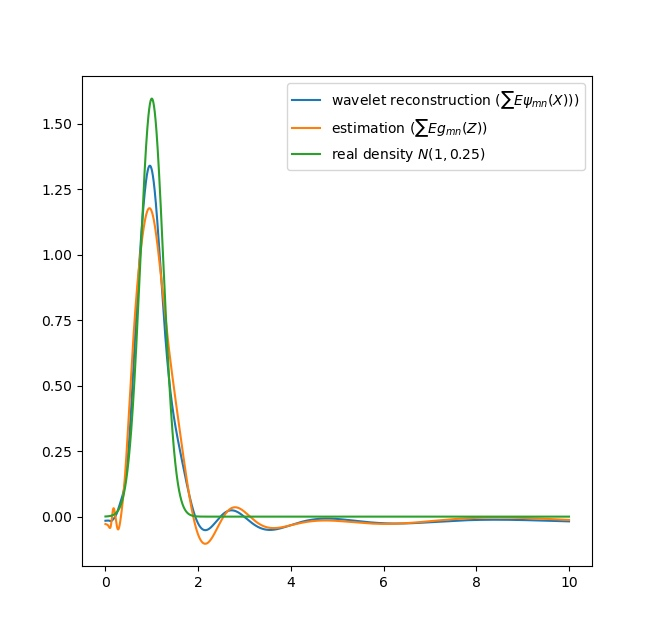
\includegraphics[width=\textwidth]{norm}
\end{figure}

\begin{figure}[h]
    \caption{$X \sim \exp(1)$}
    \centering
    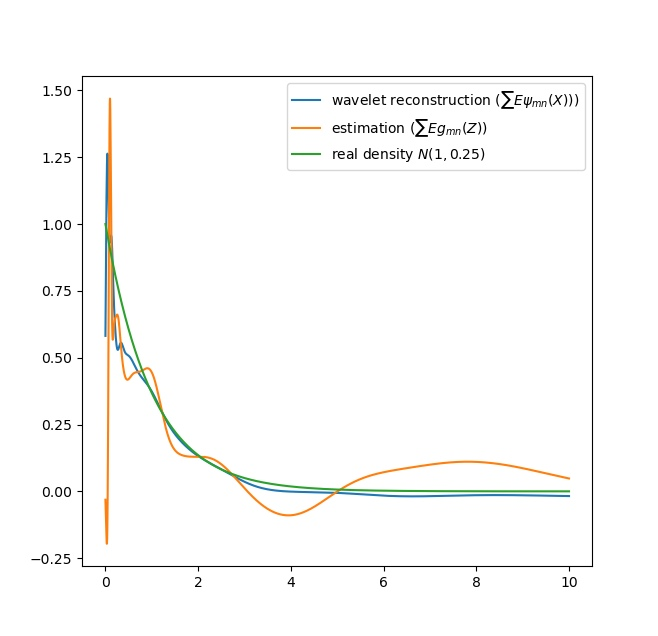
\includegraphics[width=\textwidth]{exp}
\end{figure}

\begin{figure}[h]
    \caption{$X \sim \chi^2_5$}
    \centering
    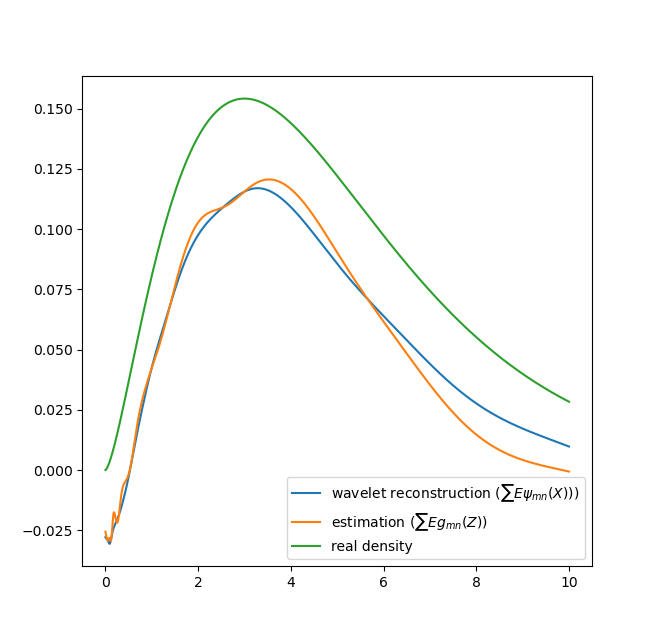
\includegraphics[width=\textwidth]{chisq}
\end{figure}
\section{Правильная часть ряда Лорана для $f(z) = e^{az} e^{-1/(2s^2)} e^{n/s}$}
\begin{Th*}
Пусть $k \ge 0$; пусть
\[
    f(z) = e^{az} e^{-1/(2s^2)} e^{b/z}
\]
Тогда $k$-й член ряда Лорана для $f$ равен
\[
    \sum_{l=0}^{\infty}
    \sum_{m=0}^{\infty} \frac{a^{2m+k+l} / \left( -2 \right)^m}{(2m+k+l)!\,m!} \\
    \frac{n^l}{l!}
\]
\end{Th*}
\begin{proof}
Определим
\begin{align*}
    & g(t) = e^{az} e^{-1/(2s^2)} \\
    & h(t) = e^{b/z}
\end{align*}
Обе функции голоморфны в $\CC \setminus \{0\}$. Поэтому их ряды сходятся абсолютны и мы можем умножить ряды по Коши, чтобы получить ряд Лорана для $f$.

У функции $e^{n/s}$ правильная часть константна.
Поэтому, согласно теореме о правильной части произведения голоморфной функции и функции с константной правильной частью, 
нам достаточно знать только правильную часть разложения функции $g$, которую мы нашли в предыдущей теореме.

Пусть $\{\alpha_n\}_{n=-\infty}^\infty$ --- коэффициенты для $g$, а $\{\beta_n\}_{n=-\infty}^0$ --- коэффициенты для $h$, а $\{\gamma_n\}_{n=-\infty}^\infty$ --- коэффициенты $f$.
Для наглядности, приведем формулу $k$-го члена их произведения, где $k \ge 0$:
\[
    \gamma_k =
    \sum_{l=-\infty}^{0} \alpha_{k-l} \beta_l =
    \sum_{l=0}^{\infty} \alpha_{k+l} \beta_{-l}
\]
Приведем также формулы для $\alpha_k$ и $\beta_{-k}$:
\begin{align*}
    & \alpha_k = \sum_{m=0}^{\infty} \frac{a^{2m+k} / \left( -2 \right)^m}{(2m+k)!\,m!} \\
    & \beta_{-k} = \frac{n^k}{k!}
\end{align*}
Подставим $\alpha_k$ и $\beta_{-k}$ в формулу для $\gamma_k$:
\[
    \gamma_k =
    \sum_{l=0}^{\infty} \alpha_{k+l} \beta_{-l} =
%
    \sum_{l=0}^{\infty}
    \sum_{m=0}^{\infty} \frac{a^{2m+k+l} / \left( -2 \right)^m}{(2m+k+l)!\,m!} \\
    \frac{n^l}{l!}
\]
\end{proof}

%
\end{document}
